\documentclass{article}

\usepackage[latin1]{inputenc}
\usepackage{tikz}

% GNUPLOT required
\begin{document}
\pagestyle{empty}


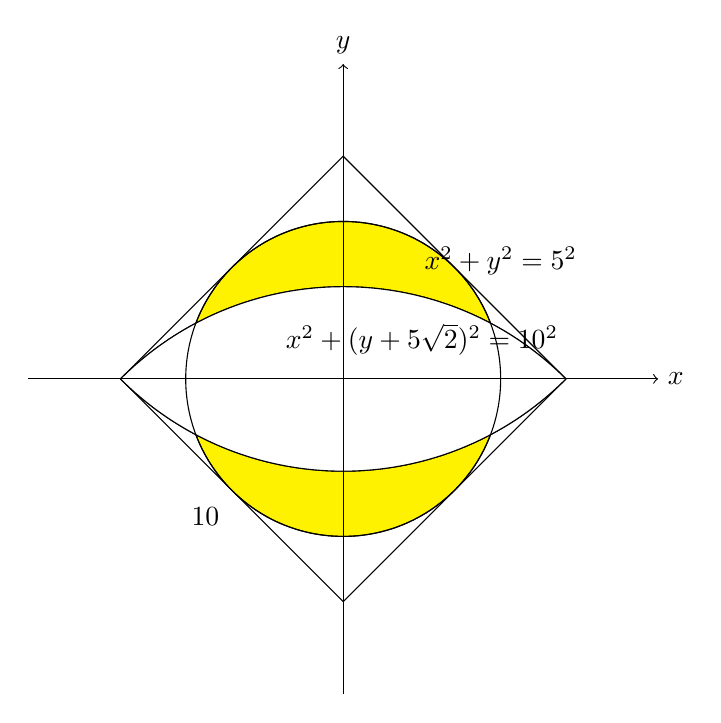
\begin{tikzpicture}
    \begin{scope}[rotate=-45]
        \draw (2, 2) rectangle (-2, -2);
        \filldraw[fill=yellow,even odd rule]
            (2, 2) arc (90:180:4) (-2, -2) arc (270:360:4)
            (2, 0) arc (0:-360:2);
        \filldraw[fill=white]
            (2, 2) arc (90:180:4) (-2, -2) arc (270:360:4);
        \draw (2, 2) (2, 0) arc (0:-360:2);
    \end{scope}
    \draw[->] (-4,0) -- (4,0) node[right] {$x$};
    \draw[->] (0,-4) -- (0,4) node[above] {$y$};
    \draw (1,0.5) node {$x^2+(y+5\sqrt{2})^2=10^2$};
    \draw (2,1.5) node {$x^2+y^2=5^2$};
    \draw (-1.75,-1.75) node {$10$};
\end{tikzpicture}

\end{document}
